% Scientific Reports layout-clean manuscript.
% Paste the current manuscript text into the marked section blocks without rewriting content.
\documentclass[fleqn,10pt]{wlscirep}

\usepackage[utf8]{inputenc}
\usepackage[T1]{fontenc}
\usepackage{graphicx}
\usepackage{booktabs}
\usepackage{array}
\usepackage{tabularx}
\usepackage{makecell}
\usepackage{multirow}
\usepackage{siunitx}
\usepackage{amsmath,amssymb}
\usepackage{placeins}
\usepackage{etoolbox}
\usepackage{xurl}

\graphicspath{{figures/}{../reports/final_results/figures/}}

\sisetup{
  detect-all,
  group-digits=false,
  table-number-alignment=center,
  round-mode=places,
  round-precision=4
}

\setlength{\tabcolsep}{4.5pt}
\renewcommand{\arraystretch}{1.12}
\AtBeginEnvironment{table}{\small}
\AtBeginEnvironment{table*}{\small}

\newcommand{\ours}{Ours}
\newcommand{\loraonly}{LoRA-only}
\newcommand{\ipadapter}{IP-Adapter only}
\newcommand{\blankiou}{Blank IoU}
\newcommand{\blankssim}{Blank SSIM}

\title{Hierarchical Structure and Style-Coordinated Diffusion for Controllable Chinese Landscape Painting Generation}

\author[1,*]{Alice Author}
\author[2]{Bob Author}
\author[1,2,+]{Christine Author}
\author[2,+]{Derek Author}
\affil[1]{Affiliation, department, city, postcode, country}
\affil[2]{Affiliation, department, city, postcode, country}
\affil[*]{corresponding.author@email.example}
\affil[+]{these authors contributed equally to this work}

%\keywords{Chinese landscape painting, diffusion models, controllable generation, hierarchical structure, style prompting}

\begin{abstract}
% Paste the original abstract here unchanged.
\end{abstract}

\begin{document}
\flushbottom
\maketitle
\thispagestyle{empty}

% Main text starts here. Keep unnumbered section commands for Scientific Reports.
% Recommended order:
% Introduction
% Related Work
% Culture-Aware Hierarchical Diffusion Framework
% Experiments and Results
% Discussion
% Data availability
% Code availability
% References
% Acknowledgements
% Author contributions statement
% Additional information

\section*{Introduction}
% Paste the original Introduction here unchanged.

% Figure 1 placeholder:
% Keep this block only after figure1_motivation_overview.pdf/png is available.
% \begin{figure}[t]
% \centering
% \includegraphics[width=\linewidth]{figure1_motivation_overview}
% \caption{\textbf{Motivation and overview of controllable Chinese landscape painting generation.}
% Paste the original caption here unchanged.}
% \label{fig:motivation-overview}
% \end{figure}

\section*{Related Work}
% Paste the original Related Work here unchanged.

\section*{Culture-Aware Hierarchical Diffusion Framework}
% Paste the original method section here unchanged.

% Figure 2 placeholder:
% Keep this block only after figure2_method_framework.pdf/png is available.
% \begin{figure*}[t]
% \centering
% \includegraphics[width=\textwidth]{figure2_method_framework}
% \caption{\textbf{Overview of the proposed hierarchical structure and style-coordinated diffusion framework.}
% Paste the original caption here unchanged.}
% \label{fig:method-framework}
% \end{figure*}

\section*{Experiments and Results}
% Paste the original Experiments and Results section here unchanged.
% Use the formatted table/figure blocks below to replace only the raw LaTeX float blocks.

\begin{table*}[t]
\centering
\caption{\textbf{Main quantitative comparison on fidelity, alignment, preference, and diversity metrics.}
The proposed method achieves the best FID and KID, indicating stronger target-domain distribution matching for Chinese landscape painting generation. IP-Adapter-only obtains the highest CLIPScore, PickScore, HPSv2, and LPIPS, suggesting that reference-image conditioning remains strong on general semantic-alignment and preference-oriented metrics.}
\label{tab:main-fidelity-preference}
\begin{tabularx}{\textwidth}{l *{6}{>{\centering\arraybackslash}X}}
\toprule
\textbf{Method} & \textbf{FID}$\downarrow$ & \textbf{KID}$\downarrow$ & \textbf{CLIPScore}$\uparrow$ & \textbf{PickScore}$\uparrow$ & \textbf{HPSv2}$\uparrow$ & \textbf{LPIPS}$\uparrow$ \\
\midrule
ControlNet & 265.89 & 0.1841 & 0.3414 & 19.97 & 0.1939 & 0.4916 \\
IP-Adapter only & 213.32 & 0.1095 & \textbf{0.3559} & \textbf{20.19} & \textbf{0.2044} & \textbf{0.5333} \\
LoRA-only & $273.40 \pm 26.12$ & $0.2287 \pm 0.0611$ & $0.3349 \pm 0.0074$ & $19.49 \pm 0.26$ & $0.1368 \pm 0.0086$ & $0.3819 \pm 0.0132$ \\
Ours & $\textbf{169.16} \pm \textbf{5.68}$ & $\textbf{0.0614} \pm \textbf{0.0050}$ & $0.3288 \pm 0.0016$ & $19.59 \pm 0.07$ & $0.1603 \pm 0.0048$ & $0.4790 \pm 0.0045$ \\
\bottomrule
\end{tabularx}
\end{table*}

\begin{table}[t]
\centering
\caption{\textbf{Style and structure-related evaluation.}
The proposed method obtains the highest style accuracy and blank-space IoU, while ControlNet achieves the highest edge consistency. This suggests that ControlNet is stronger at hard edge adherence, whereas the proposed method provides a more balanced structure-style generation behavior.}
\label{tab:main-structure-style}
\begin{tabularx}{\linewidth}{l *{4}{>{\centering\arraybackslash}X}}
\toprule
\textbf{Method} & \textbf{Style Acc.}$\uparrow$ & \textbf{Edge Cons.}$\uparrow$ & \textbf{Blank IoU}$\uparrow$ & \textbf{Blank SSIM}$\uparrow$ \\
\midrule
ControlNet & 0.4217 & \textbf{0.0685} & 0.0077 & 0.7031 \\
IP-Adapter only & 0.5422 & 0.0383 & 0.0051 & 0.6998 \\
LoRA-only & $0.3373 \pm 0.0000$ & $0.0015 \pm 0.0005$ & $0.0000 \pm 0.0000$ & $\textbf{0.7126} \pm 0.0000$ \\
Ours & $\textbf{0.5783} \pm \textbf{0.0197}$ & $0.0347 \pm 0.0006$ & $\textbf{0.0140} \pm \textbf{0.0039}$ & $0.7096 \pm 0.0015$ \\
\bottomrule
\end{tabularx}
\end{table}

\begin{figure*}[t]
\centering
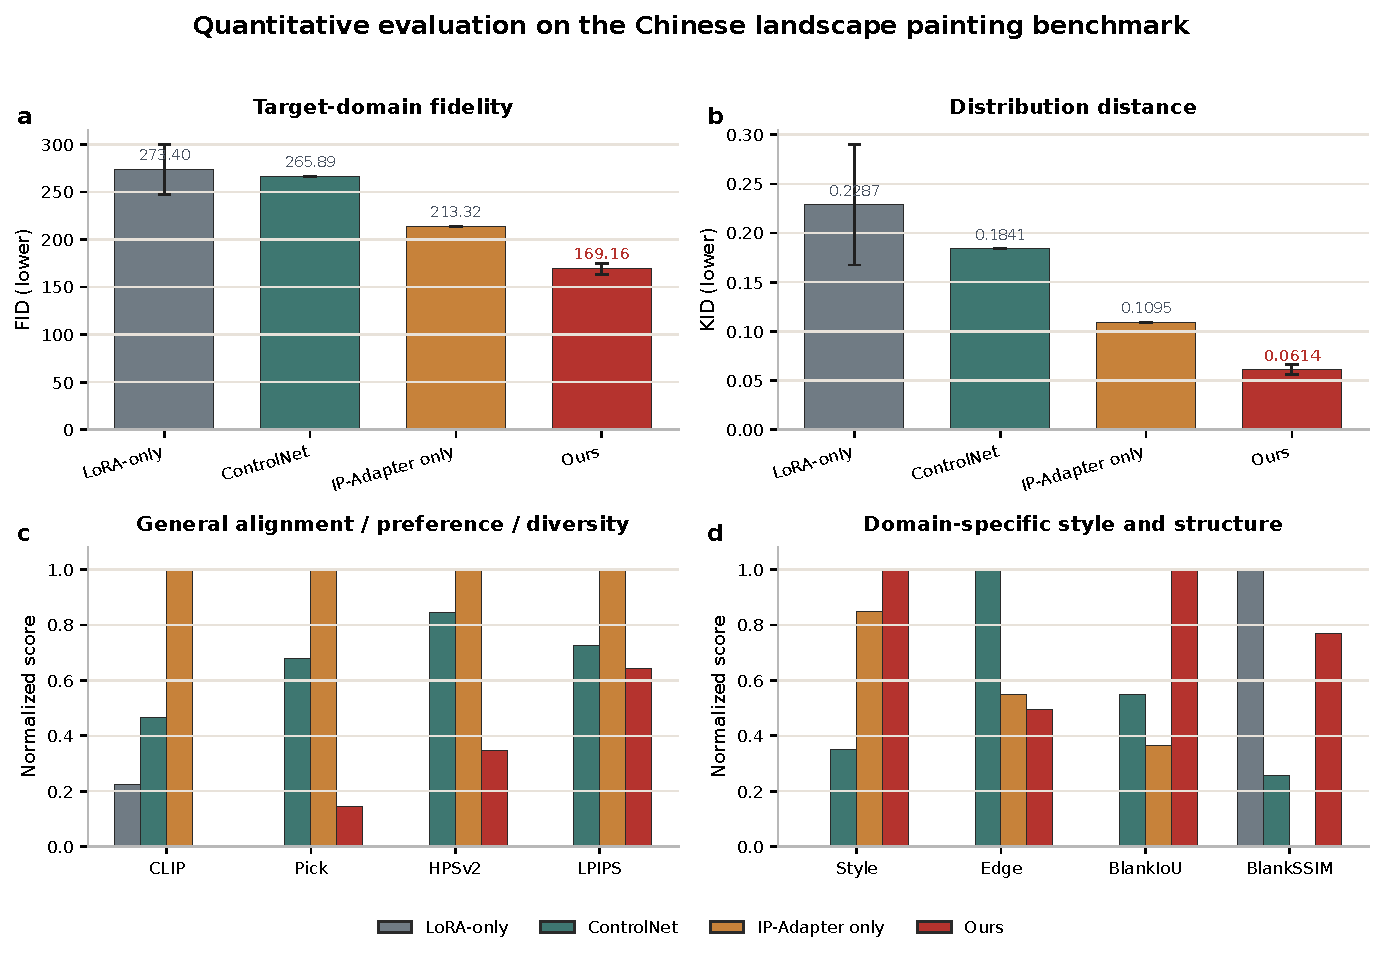
\includegraphics[width=\textwidth]{figure6_quantitative_summary}
\caption{\textbf{Quantitative evaluation on the Chinese landscape painting benchmark.}
\textbf{(a)} FID comparison. Lower values indicate better target-domain fidelity.
\textbf{(b)} KID comparison. Lower values indicate smaller distribution distance.
\textbf{(c)} Direction-aware normalized comparison of general alignment, preference, and diversity metrics.
\textbf{(d)} Direction-aware normalized comparison of domain-specific style and structure metrics.
For panels (c) and (d), all metrics are min--max normalized after direction correction, so that higher values indicate better performance. The proposed method achieves the strongest distribution fidelity and performs best on style accuracy and Blank IoU, while IP-Adapter-only performs better on several general preference-oriented metrics and ControlNet obtains the highest edge consistency.}
\label{fig:quantitative-summary}
\end{figure*}

\begin{figure*}[t]
\centering
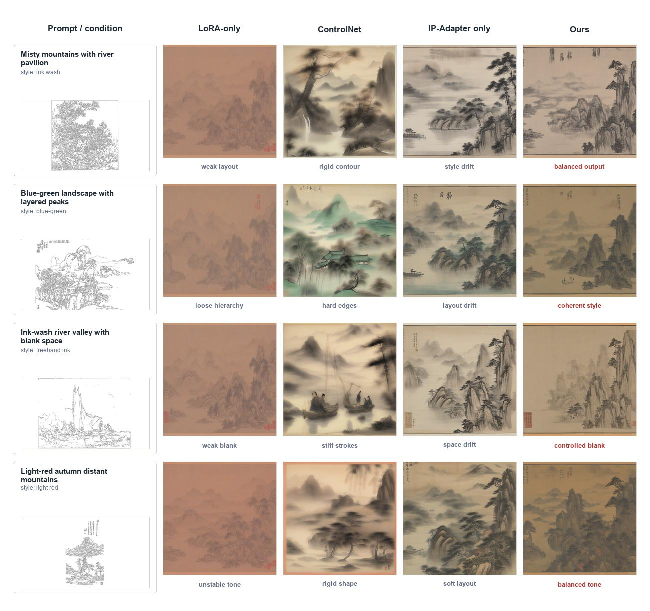
\includegraphics[width=\textwidth]{figure4_qualitative_comparison}
\caption{\textbf{Main qualitative comparison on the held-out test set.}
Each row shows one representative test case under matched prompt and structure conditions. LoRA-only learns part of the Chinese landscape painting appearance but often shows weak layout control. ControlNet follows structural cues more strongly but tends to produce rigid contours. IP-Adapter-only provides stronger style cues but may exhibit layout drift. The proposed method achieves a more balanced result in compositional hierarchy, blank-space organization, brush-and-ink consistency, and target-domain fidelity.}
\label{fig:qualitative-comparison}
\end{figure*}

\begin{figure*}[t]
\centering

\includegraphics[width=\textwidth]{figure5_structure_controllability}
\caption{\textbf{Structure controllability visualization under a unified prompt.}
All examples use the same text prompt but different hierarchical structure conditions. The left column shows the input structure maps, and the right column shows the corresponding generated outputs from the proposed method. The selected cases cover a large upper blank space, dominant central peak, left-heavy mountain composition, and lower-right foreground structure. Blue dashed boxes indicate blank-space or depth-related regions, while orange dashed boxes indicate the main compositional or foreground regions. The results show that the proposed hierarchical structure condition can guide composition placement, blank-space organization, and spatial hierarchy.}
\label{fig:structure-controllability}
\end{figure*}

\begin{figure*}[t]
\centering

\includegraphics[width=\textwidth]{figure7_tradeoff_and_significance}
\caption{\textbf{Trade-off and significance analysis.}
\textbf{(a)} Fidelity-style trade-off across compared methods. The horizontal axis is inverted so that points further right indicate better FID. Marker size encodes LPIPS diversity.
\textbf{(b)} Paired Wilcoxon significance analysis between the proposed method and LoRA-only on 83 paired test samples. Red bars indicate metrics where the proposed method is higher, and gray bars indicate metrics where LoRA-only is higher.}
\label{fig:tradeoff-significance}
\end{figure*}

\FloatBarrier

\section*{Discussion}
% Paste the original Discussion here unchanged.

\section*{Data availability}
% Add the dataset availability statement here.

\section*{Code availability}
% Add the code availability statement here.

\bibliography{sample}

\section*{Acknowledgements}
% Add acknowledgements here if applicable.

\section*{Author contributions statement}
A.A. conceived the experiment(s), A.A. and B.A. conducted the experiment(s), C.A. and D.A. analysed the results. All authors reviewed the manuscript.

\section*{Additional information}
\textbf{Competing interests:} The authors declare no competing interests.

\end{document}
